\documentclass[twoside]{book}

% Packages required by doxygen
\usepackage{fixltx2e}
\usepackage{calc}
\usepackage{doxygen}
\usepackage[export]{adjustbox} % also loads graphicx
\usepackage{graphicx}
\usepackage[utf8]{inputenc}
\usepackage{makeidx}
\usepackage{multicol}
\usepackage{multirow}
\PassOptionsToPackage{warn}{textcomp}
\usepackage{textcomp}
\usepackage[nointegrals]{wasysym}
\usepackage[table]{xcolor}

% Font selection
\usepackage[T1]{fontenc}
\usepackage[scaled=.90]{helvet}
\usepackage{courier}
\usepackage{amssymb}
\usepackage{sectsty}
\renewcommand{\familydefault}{\sfdefault}
\allsectionsfont{%
  \fontseries{bc}\selectfont%
  \color{darkgray}%
}
\renewcommand{\DoxyLabelFont}{%
  \fontseries{bc}\selectfont%
  \color{darkgray}%
}
\newcommand{\+}{\discretionary{\mbox{\scriptsize$\hookleftarrow$}}{}{}}

% Page & text layout
\usepackage{geometry}
\geometry{%
  a4paper,%
  top=2.5cm,%
  bottom=2.5cm,%
  left=2.5cm,%
  right=2.5cm%
}
\tolerance=750
\hfuzz=15pt
\hbadness=750
\setlength{\emergencystretch}{15pt}
\setlength{\parindent}{0cm}
\setlength{\parskip}{3ex plus 2ex minus 2ex}
\makeatletter
\renewcommand{\paragraph}{%
  \@startsection{paragraph}{4}{0ex}{-1.0ex}{1.0ex}{%
    \normalfont\normalsize\bfseries\SS@parafont%
  }%
}
\renewcommand{\subparagraph}{%
  \@startsection{subparagraph}{5}{0ex}{-1.0ex}{1.0ex}{%
    \normalfont\normalsize\bfseries\SS@subparafont%
  }%
}
\makeatother

% Headers & footers
\usepackage{fancyhdr}
\pagestyle{fancyplain}
\fancyhead[LE]{\fancyplain{}{\bfseries\thepage}}
\fancyhead[CE]{\fancyplain{}{}}
\fancyhead[RE]{\fancyplain{}{\bfseries\leftmark}}
\fancyhead[LO]{\fancyplain{}{\bfseries\rightmark}}
\fancyhead[CO]{\fancyplain{}{}}
\fancyhead[RO]{\fancyplain{}{\bfseries\thepage}}
\fancyfoot[LE]{\fancyplain{}{}}
\fancyfoot[CE]{\fancyplain{}{}}
\fancyfoot[RE]{\fancyplain{}{\bfseries\scriptsize Generated by Doxygen }}
\fancyfoot[LO]{\fancyplain{}{\bfseries\scriptsize Generated by Doxygen }}
\fancyfoot[CO]{\fancyplain{}{}}
\fancyfoot[RO]{\fancyplain{}{}}
\renewcommand{\footrulewidth}{0.4pt}
\renewcommand{\chaptermark}[1]{%
  \markboth{#1}{}%
}
\renewcommand{\sectionmark}[1]{%
  \markright{\thesection\ #1}%
}

% Indices & bibliography
\usepackage{natbib}
\usepackage[titles]{tocloft}
\setcounter{tocdepth}{3}
\setcounter{secnumdepth}{5}
\makeindex

% Hyperlinks (required, but should be loaded last)
\usepackage{ifpdf}
\ifpdf
  \usepackage[pdftex,pagebackref=true]{hyperref}
\else
  \usepackage[ps2pdf,pagebackref=true]{hyperref}
\fi
\hypersetup{%
  colorlinks=true,%
  linkcolor=blue,%
  citecolor=blue,%
  unicode%
}

% Custom commands
\newcommand{\clearemptydoublepage}{%
  \newpage{\pagestyle{empty}\cleardoublepage}%
}

\usepackage{caption}
\captionsetup{labelsep=space,justification=centering,font={bf},singlelinecheck=off,skip=4pt,position=top}

%===== C O N T E N T S =====

\begin{document}

% Titlepage & ToC
\hypersetup{pageanchor=false,
             bookmarksnumbered=true,
             pdfencoding=unicode
            }
\pagenumbering{alph}
\begin{titlepage}
\vspace*{7cm}
\begin{center}%
{\Large Numerical Integration }\\
\vspace*{1cm}
{\large Generated by Doxygen 1.8.13}\\
\end{center}
\end{titlepage}
\clearemptydoublepage
\pagenumbering{roman}
\tableofcontents
\clearemptydoublepage
\pagenumbering{arabic}
\hypersetup{pageanchor=true}

%--- Begin generated contents ---
\chapter{Project 5 -\/ Numerical Integration}
\label{md__r_e_a_d_m_e}
\Hypertarget{md__r_e_a_d_m_e}
{\itshape \href{https://gitlab.epfl.ch/majoor/project-5-numerical-integration}{\tt https\+://gitlab.\+epfl.\+ch/majoor/project-\/5-\/numerical-\/integration}}

\subsubsection*{Compiling the Program for the First Time}

The following steps should be undertaken to run our code
\begin{DoxyItemize}
\item clone the repository with 
\begin{DoxyCode}
git clone git@gitlab.epfl.ch:majoor/project-5-numerical-integration.git
\end{DoxyCode}

\item move to the cloned directory 
\begin{DoxyCode}
cd project-5-numerical-integration/
\end{DoxyCode}

\item fetch the submodules (Eigen and Googletest) using 
\begin{DoxyCode}
git submodule update --init
\end{DoxyCode}

\item build the executable using C\+M\+A\+KE 
\begin{DoxyCode}
mkdir build
cd build
cmake ..
make
\end{DoxyCode}

\item run the executable 
\begin{DoxyCode}
./integration
\end{DoxyCode}

\end{DoxyItemize}

This code will produce the following output\+: 
\begin{DoxyCode}
Successfully opened file ../readfile.txt

---Input Data---

D: 2
m: 2
boundsX: 
1 2
6 7
boundsY: 
  5   6
  8 9.5
noSteps: 
10 11
 3 10
coefficients: 
  (1,1) (15,-5) (-2,11) (1,3.6)
 (5,-6)  (10,1)   (0,0)   (0,0)

---Integration Methods---

MidpointFormula:
[ 199.819 + 388.072i,
125 + -3.75i ]

TrapezoidalRule:
[ 202.09 + 390.886i,
125.909 + -3.65909i ]

SimpsonsRule:
[ 199.833 + 388.125i,
125 + -3.75i ]
\end{DoxyCode}


\subsubsection*{Configuring the Program}

To run the program with different integrals and different domains of integration, the input file {\ttfamily readfile.\+txt} can be configured. An example of the format required is shown below\+:



The first line details the length of inputs the program should expect. The lines (a), (b), (c) and (d) are then read as follows\+:
\begin{DoxyItemize}
\item $\ast$(a)$\ast$ first domain is between x=1 and x=2, y=5 and y=6 and the integration method undergoes 10 steps in the x direction and 11 steps in the y direction
\item $\ast$(b)$\ast$ first domain is between x=6 and x=7, y=8 and y=9.\+5 and the integration method undergoes 3 steps in the x direction and 10 steps in the y direction
\item $\ast$(c)$\ast$ first function output reads 1+1i + (15-\/5i)x + (-\/2+11i)y + (1+3.6i)x$^\wedge$2
\item $\ast$(d)$\ast$ second function output reads 5-\/6i + (19+1i)x + (0+0i)y + (0+0i)x$^\wedge$2
\end{DoxyItemize}

{\itshape Note\+: to configure a 1D integration task, it suffices to set all coefficients of y$^\wedge$n terms to 0, and to set the y-\/bounds to differ by 1.}

\subsubsection*{Typical Program Usage}

A typical execution would be to edit the configuration file {\ttfamily readfile.\+txt} to indicate a new integration problem, and then to simply rerun the program with {\ttfamily ./integration} and view the results of the methods.

\subsubsection*{Program Features}


\begin{DoxyItemize}
\item Reads arbitrary input from file
\item Implementation of 3 integration methods in 2D and 1D
\item Error handling
\item Individual testing of all features
\item Documentation of all code
\item Extensible code due to polymorphic approach
\end{DoxyItemize}

\subsubsection*{Documentation}

To generate documentation, Doxygen is required to be installed on the system, and can be downloaded \href{https://www.doxygen.nl/download.html}{\tt here}.
\begin{DoxyItemize}
\item To generate the documentation, the command 
\begin{DoxyCode}
doxygen Doxyfile
\end{DoxyCode}
 should be run from the root directory.
\item Documentation can be viewed in the {\ttfamily html/} folder. To open the documentation, once can execute the following\+: 
\begin{DoxyCode}
xdg-open html/index.html
\end{DoxyCode}

\end{DoxyItemize}

\subsubsection*{Tests}

To execute tests, it suffices to run 
\begin{DoxyCode}
./Tests
\end{DoxyCode}
 from the {\ttfamily build/} directory.

Two types of test are run using googletest \+:
\begin{DoxyItemize}
\item Tests of the text file reader
\item Tests of the integration methods
\end{DoxyItemize}

For the reader, we execute a few death tests to ensure that the first inputs are asserted to be positive.

For the integration, we run tests on polynomials of 4 values of l (l is defined above).
\begin{DoxyItemize}
\item For l=1, we integrate a constant function and expect an exact solution for all 3 methods.
\item For l=3, we expect an exact solution for midpoint and Simpson but an approximate solution for trapezoidal.
\item For l=6, we expect an exact solution for Simpson but an approximate solution for midpoint and trapezoidal.
\item For l=9, we expect an approximate solution for all 3 methods.
\end{DoxyItemize}

\subsubsection*{Current Issues/\+Limitations}


\begin{DoxyItemize}
\item Limited error handling
\item Wasteful to have {\ttfamily Eigen\+::\+Vector\+Xcd ($\ast$f)(double x, double y, Eigen\+::\+Matrix\+Xcd \&coeff)} take {\ttfamily \&coeff} as input
\item No specifiers const and unsigned
\item No use of override
\end{DoxyItemize}

\subsubsection*{Suggestions for Future Improvement}


\begin{DoxyItemize}
\item Extension to 3D or higher
\item Read input from other file structures
\item Store result in a file 
\end{DoxyItemize}
\chapter{Hierarchical Index}
\section{Class Hierarchy}
This inheritance list is sorted roughly, but not completely, alphabetically\+:\begin{DoxyCompactList}
\item \contentsline{section}{Abstract\+Integration\+Method}{\pageref{class_abstract_integration_method}}{}
\begin{DoxyCompactList}
\item \contentsline{section}{Midpoint\+Formula}{\pageref{class_midpoint_formula}}{}
\item \contentsline{section}{Simpsons\+Rule}{\pageref{class_simpsons_rule}}{}
\item \contentsline{section}{Trapezoidal\+Rule}{\pageref{class_trapezoidal_rule}}{}
\end{DoxyCompactList}
\item \contentsline{section}{Abstract\+Reader}{\pageref{class_abstract_reader}}{}
\begin{DoxyCompactList}
\item \contentsline{section}{Txt\+Reader}{\pageref{class_txt_reader}}{}
\end{DoxyCompactList}
\item \contentsline{section}{Data}{\pageref{struct_data}}{}
\end{DoxyCompactList}

\chapter{Class Index}
\section{Class List}
Here are the classes, structs, unions and interfaces with brief descriptions\+:\begin{DoxyCompactList}
\item\contentsline{section}{\hyperlink{class_abstract_integration_method}{Abstract\+Integration\+Method} \\*Abstract class for implementation of integration algorithms }{\pageref{class_abstract_integration_method}}{}
\item\contentsline{section}{\hyperlink{class_abstract_reader}{Abstract\+Reader} \\*Abstract class for implementation of file reading }{\pageref{class_abstract_reader}}{}
\item\contentsline{section}{\hyperlink{struct_data}{Data} \\*Struct storing data for the integral computation }{\pageref{struct_data}}{}
\item\contentsline{section}{\hyperlink{class_midpoint_formula}{Midpoint\+Formula} \\*Class implementing the Midpoint Formula approximation of integrals in 2D or 1D }{\pageref{class_midpoint_formula}}{}
\item\contentsline{section}{\hyperlink{class_simpsons_rule}{Simpsons\+Rule} \\*Class implementing the Simpson\textquotesingle{}s Rule approximation of integrals in 2D or 1D }{\pageref{class_simpsons_rule}}{}
\item\contentsline{section}{\hyperlink{class_trapezoidal_rule}{Trapezoidal\+Rule} \\*Class implementing the Trapezoidal Rule approximation of integrals in 2D or 1D }{\pageref{class_trapezoidal_rule}}{}
\item\contentsline{section}{\hyperlink{class_txt_reader}{Txt\+Reader} \\*Class implementing reading data from T\+XT riles }{\pageref{class_txt_reader}}{}
\end{DoxyCompactList}

\chapter{Class Documentation}
\hypertarget{class_abstract_integration_method}{}\section{Abstract\+Integration\+Method Class Reference}
\label{class_abstract_integration_method}\index{Abstract\+Integration\+Method@{Abstract\+Integration\+Method}}


Abstract class for implementation of integration algorithms.  




{\ttfamily \#include $<$Abstract\+Integration\+Method.\+h$>$}



Inheritance diagram for Abstract\+Integration\+Method\+:\nopagebreak
\begin{figure}[H]
\begin{center}
\leavevmode
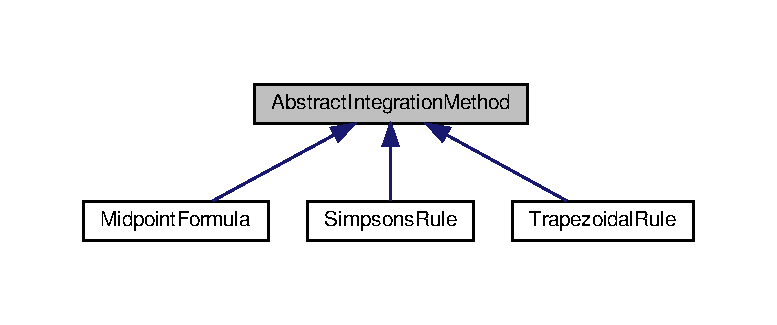
\includegraphics[width=350pt]{class_abstract_integration_method__inherit__graph}
\end{center}
\end{figure}


Collaboration diagram for Abstract\+Integration\+Method\+:\nopagebreak
\begin{figure}[H]
\begin{center}
\leavevmode
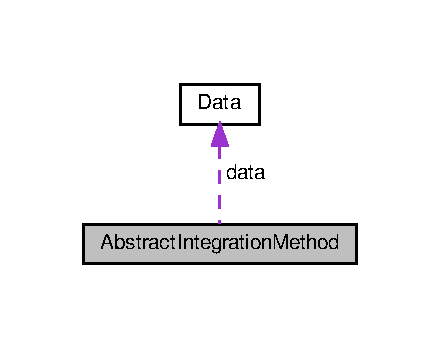
\includegraphics[width=211pt]{class_abstract_integration_method__coll__graph}
\end{center}
\end{figure}
\subsection*{Public Member Functions}
\begin{DoxyCompactItemize}
\item 
\mbox{\Hypertarget{class_abstract_integration_method_ac9094172e42a206908a2724cb25159c0}\label{class_abstract_integration_method_ac9094172e42a206908a2724cb25159c0}} 
\hyperlink{class_abstract_integration_method_ac9094172e42a206908a2724cb25159c0}{Abstract\+Integration\+Method} (\hyperlink{struct_data}{Data} \&data, Eigen\+::\+Vector\+Xcd($\ast$function)(double x, double y, Eigen\+::\+Matrix\+Xcd \&coeff))
\begin{DoxyCompactList}\small\item\em Initialiser setting the data as a \hyperlink{struct_data}{Data} struct and also the function to integrate. \end{DoxyCompactList}\item 
virtual Eigen\+::\+Vector\+Xcd \hyperlink{class_abstract_integration_method_af76e5bdce7d0b139d07e920fa29c1c34}{Solve} ()=0
\begin{DoxyCompactList}\small\item\em Method to compute approximate value of the 2D or 1D integral. \end{DoxyCompactList}\end{DoxyCompactItemize}
\subsection*{Protected Attributes}
\begin{DoxyCompactItemize}
\item 
\mbox{\Hypertarget{class_abstract_integration_method_a534b5ff7dfbccc1332cfbe66e817b389}\label{class_abstract_integration_method_a534b5ff7dfbccc1332cfbe66e817b389}} 
\hyperlink{struct_data}{Data} {\bfseries data}
\item 
\mbox{\Hypertarget{class_abstract_integration_method_af94033e3acb2f881e9973480809e2e2f}\label{class_abstract_integration_method_af94033e3acb2f881e9973480809e2e2f}} 
Eigen\+::\+Vector\+Xcd($\ast$ {\bfseries f} )(double x, double y, Eigen\+::\+Matrix\+Xcd \&coeff)
\end{DoxyCompactItemize}


\subsection{Detailed Description}
Abstract class for implementation of integration algorithms. 

Takes as input a \hyperlink{struct_data}{Data} struct and implements a \hyperlink{class_abstract_integration_method_af76e5bdce7d0b139d07e920fa29c1c34}{Solve()} method returning the approximation of the 2D or 1D integral 

\subsection{Member Function Documentation}
\mbox{\Hypertarget{class_abstract_integration_method_af76e5bdce7d0b139d07e920fa29c1c34}\label{class_abstract_integration_method_af76e5bdce7d0b139d07e920fa29c1c34}} 
\index{Abstract\+Integration\+Method@{Abstract\+Integration\+Method}!Solve@{Solve}}
\index{Solve@{Solve}!Abstract\+Integration\+Method@{Abstract\+Integration\+Method}}
\subsubsection{\texorpdfstring{Solve()}{Solve()}}
{\footnotesize\ttfamily virtual Eigen\+::\+Vector\+Xcd Abstract\+Integration\+Method\+::\+Solve (\begin{DoxyParamCaption}{ }\end{DoxyParamCaption})\hspace{0.3cm}{\ttfamily [pure virtual]}}



Method to compute approximate value of the 2D or 1D integral. 

\begin{DoxyReturn}{Returns}
The complex vector result of the integral approximation 
\end{DoxyReturn}


Implemented in \hyperlink{class_simpsons_rule_a9925b07e44be9fc1644d3cbeb742078c}{Simpsons\+Rule}, \hyperlink{class_trapezoidal_rule_ae822d86948bdc8876bf524cd620e11b8}{Trapezoidal\+Rule}, and \hyperlink{class_midpoint_formula_add437323dfb0bc181b0051c5aaf80ba7}{Midpoint\+Formula}.



The documentation for this class was generated from the following files\+:\begin{DoxyCompactItemize}
\item 
Abstract\+Integration\+Method.\+h\item 
Abstract\+Integration\+Method.\+cpp\end{DoxyCompactItemize}

\hypertarget{class_abstract_reader}{}\section{Abstract\+Reader Class Reference}
\label{class_abstract_reader}\index{Abstract\+Reader@{Abstract\+Reader}}


Abstract class for implementation of file reading.  




{\ttfamily \#include $<$Abstract\+Reader.\+h$>$}



Inheritance diagram for Abstract\+Reader\+:\nopagebreak
\begin{figure}[H]
\begin{center}
\leavevmode
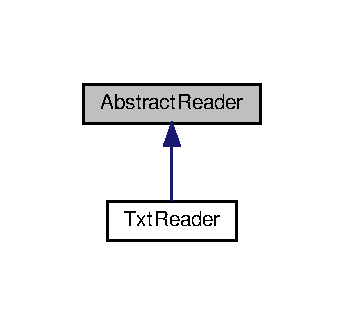
\includegraphics[width=165pt]{class_abstract_reader__inherit__graph}
\end{center}
\end{figure}
\subsection*{Public Member Functions}
\begin{DoxyCompactItemize}
\item 
\mbox{\Hypertarget{class_abstract_reader_af7d4391a1d75538c6bb406c00acabd30}\label{class_abstract_reader_af7d4391a1d75538c6bb406c00acabd30}} 
\hyperlink{class_abstract_reader_af7d4391a1d75538c6bb406c00acabd30}{Abstract\+Reader} (std\+::string filename)
\begin{DoxyCompactList}\small\item\em Initialiser setting filename. \end{DoxyCompactList}\item 
virtual \hyperlink{struct_data}{Data} \hyperlink{class_abstract_reader_a14b05f156920be0cfa0cabdb1c6c1267}{Output\+Data} ()=0
\begin{DoxyCompactList}\small\item\em Method to compute data as \hyperlink{struct_data}{Data} struct from file. \end{DoxyCompactList}\end{DoxyCompactItemize}
\subsection*{Protected Attributes}
\begin{DoxyCompactItemize}
\item 
\mbox{\Hypertarget{class_abstract_reader_a143f9961ba8aca61c32234a042e466ce}\label{class_abstract_reader_a143f9961ba8aca61c32234a042e466ce}} 
std\+::string {\bfseries fname}
\end{DoxyCompactItemize}


\subsection{Detailed Description}
Abstract class for implementation of file reading. 

Takes as input a filename and outputs a \hyperlink{struct_data}{Data} struct 

\subsection{Member Function Documentation}
\mbox{\Hypertarget{class_abstract_reader_a14b05f156920be0cfa0cabdb1c6c1267}\label{class_abstract_reader_a14b05f156920be0cfa0cabdb1c6c1267}} 
\index{Abstract\+Reader@{Abstract\+Reader}!Output\+Data@{Output\+Data}}
\index{Output\+Data@{Output\+Data}!Abstract\+Reader@{Abstract\+Reader}}
\subsubsection{\texorpdfstring{Output\+Data()}{OutputData()}}
{\footnotesize\ttfamily virtual \hyperlink{struct_data}{Data} Abstract\+Reader\+::\+Output\+Data (\begin{DoxyParamCaption}{ }\end{DoxyParamCaption})\hspace{0.3cm}{\ttfamily [pure virtual]}}



Method to compute data as \hyperlink{struct_data}{Data} struct from file. 

\begin{DoxyReturn}{Returns}
A \hyperlink{struct_data}{Data} object read from the the file 
\end{DoxyReturn}


Implemented in \hyperlink{class_txt_reader_a30786dcd83c2f24dd26e83cb5fd934ab}{Txt\+Reader}.



The documentation for this class was generated from the following files\+:\begin{DoxyCompactItemize}
\item 
Abstract\+Reader.\+h\item 
Abstract\+Reader.\+cpp\end{DoxyCompactItemize}

\hypertarget{struct_data}{}\section{Data Struct Reference}
\label{struct_data}\index{Data@{Data}}


Struct storing data for the integral computation.  




{\ttfamily \#include $<$Data\+Struct.\+h$>$}

\subsection*{Public Attributes}
\begin{DoxyCompactItemize}
\item 
\mbox{\Hypertarget{struct_data_a5d52cb2b68c752fa8b74b86ccb1d7e3d}\label{struct_data_a5d52cb2b68c752fa8b74b86ccb1d7e3d}} 
Eigen\+::\+Matrix\+X2d \hyperlink{struct_data_a5d52cb2b68c752fa8b74b86ccb1d7e3d}{boundsX}
\begin{DoxyCompactList}\small\item\em Matrix storing the bounds for the x-\/coordinate. \end{DoxyCompactList}\item 
\mbox{\Hypertarget{struct_data_aa34a405b70244ad387719f8d38de51ed}\label{struct_data_aa34a405b70244ad387719f8d38de51ed}} 
Eigen\+::\+Matrix\+X2d \hyperlink{struct_data_aa34a405b70244ad387719f8d38de51ed}{boundsY}
\begin{DoxyCompactList}\small\item\em Matrix storing the bounds for the y-\/coordinate. \end{DoxyCompactList}\item 
\mbox{\Hypertarget{struct_data_a97a70b84170c9d1e46705fc5a8e1db20}\label{struct_data_a97a70b84170c9d1e46705fc5a8e1db20}} 
Eigen\+::\+Matrix\+X2i \hyperlink{struct_data_a97a70b84170c9d1e46705fc5a8e1db20}{no\+Steps}
\begin{DoxyCompactList}\small\item\em Matrix the number of steps to take in the approximation. \end{DoxyCompactList}\item 
\mbox{\Hypertarget{struct_data_aa8aaf26f991decdf85559d5fa417f520}\label{struct_data_aa8aaf26f991decdf85559d5fa417f520}} 
Eigen\+::\+Matrix\+Xcd \hyperlink{struct_data_aa8aaf26f991decdf85559d5fa417f520}{coefficients}
\begin{DoxyCompactList}\small\item\em Matrix storing the polynomial coefficients specifying the function to integrate. \end{DoxyCompactList}\item 
\mbox{\Hypertarget{struct_data_afe887f8ffbf8e145e0277093134cabcc}\label{struct_data_afe887f8ffbf8e145e0277093134cabcc}} 
int \hyperlink{struct_data_afe887f8ffbf8e145e0277093134cabcc}{D}
\begin{DoxyCompactList}\small\item\em Integer storing the number of domains to integrate over. \end{DoxyCompactList}\item 
\mbox{\Hypertarget{struct_data_ab256a1176f3ba99a220c648b0c855840}\label{struct_data_ab256a1176f3ba99a220c648b0c855840}} 
int \hyperlink{struct_data_ab256a1176f3ba99a220c648b0c855840}{m}
\begin{DoxyCompactList}\small\item\em Integer storing the number of outputs of the function to integrate. \end{DoxyCompactList}\end{DoxyCompactItemize}


\subsection{Detailed Description}
Struct storing data for the integral computation. 

The documentation for this struct was generated from the following file\+:\begin{DoxyCompactItemize}
\item 
Data\+Struct.\+h\end{DoxyCompactItemize}

\hypertarget{class_midpoint_formula}{}\section{Midpoint\+Formula Class Reference}
\label{class_midpoint_formula}\index{Midpoint\+Formula@{Midpoint\+Formula}}


Class implementing the Midpoint Formula approximation of integrals in 2D or 1D.  




{\ttfamily \#include $<$Midpoint\+Formula.\+h$>$}



Inheritance diagram for Midpoint\+Formula\+:\nopagebreak
\begin{figure}[H]
\begin{center}
\leavevmode
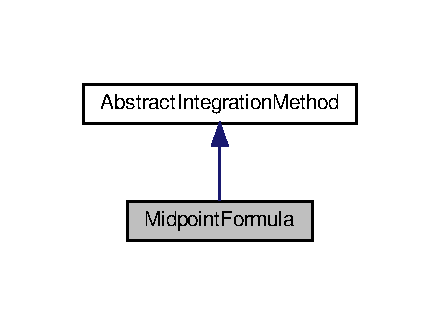
\includegraphics[width=211pt]{class_midpoint_formula__inherit__graph}
\end{center}
\end{figure}


Collaboration diagram for Midpoint\+Formula\+:\nopagebreak
\begin{figure}[H]
\begin{center}
\leavevmode
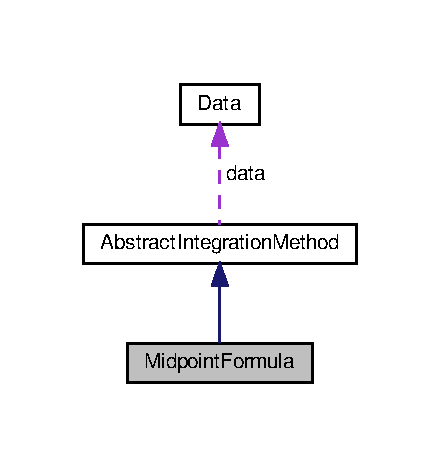
\includegraphics[width=211pt]{class_midpoint_formula__coll__graph}
\end{center}
\end{figure}
\subsection*{Public Member Functions}
\begin{DoxyCompactItemize}
\item 
\mbox{\Hypertarget{class_midpoint_formula_ad3c444776b53996d50dbf88a61c36c8c}\label{class_midpoint_formula_ad3c444776b53996d50dbf88a61c36c8c}} 
\hyperlink{class_midpoint_formula_ad3c444776b53996d50dbf88a61c36c8c}{Midpoint\+Formula} (\hyperlink{struct_data}{Data} data, Eigen\+::\+Vector\+Xcd($\ast$f)(double x, double y, Eigen\+::\+Matrix\+Xcd coeff))
\begin{DoxyCompactList}\small\item\em Initialiser setting the data as a \hyperlink{struct_data}{Data} struct and also the function to integrate. \end{DoxyCompactList}\item 
Eigen\+::\+Vector\+Xcd \hyperlink{class_midpoint_formula_add437323dfb0bc181b0051c5aaf80ba7}{Solve} ()
\begin{DoxyCompactList}\small\item\em Method to compute approximate value of the 2D or 1D integral with Midpoint Formula. \end{DoxyCompactList}\end{DoxyCompactItemize}
\subsection*{Additional Inherited Members}


\subsection{Detailed Description}
Class implementing the Midpoint Formula approximation of integrals in 2D or 1D. 

Takes as input a \hyperlink{struct_data}{Data} struct and implements a \hyperlink{class_midpoint_formula_add437323dfb0bc181b0051c5aaf80ba7}{Solve()} method returning the 2D or 1D Midpoint Formula approximation of the integral 

\subsection{Member Function Documentation}
\mbox{\Hypertarget{class_midpoint_formula_add437323dfb0bc181b0051c5aaf80ba7}\label{class_midpoint_formula_add437323dfb0bc181b0051c5aaf80ba7}} 
\index{Midpoint\+Formula@{Midpoint\+Formula}!Solve@{Solve}}
\index{Solve@{Solve}!Midpoint\+Formula@{Midpoint\+Formula}}
\subsubsection{\texorpdfstring{Solve()}{Solve()}}
{\footnotesize\ttfamily Eigen\+::\+Vector\+Xcd Midpoint\+Formula\+::\+Solve (\begin{DoxyParamCaption}{ }\end{DoxyParamCaption})\hspace{0.3cm}{\ttfamily [virtual]}}



Method to compute approximate value of the 2D or 1D integral with Midpoint Formula. 

Takes as input a \hyperlink{struct_data}{Data} struct and implements a \hyperlink{class_midpoint_formula_add437323dfb0bc181b0051c5aaf80ba7}{Solve()} method returning the 2D or 1D Midpoint Formula approximation of the integral \begin{eqnarray*} I &\approx& h_x h_y \left[ \sum_{i=1}^{n_y} \sum_{j=1}^{n_x} f\left(\frac{x_{j-1}+x_j}{2}, \frac{y_{i-1}+y_i}{2}\right) \right] \end{eqnarray*}

\begin{DoxyReturn}{Returns}
The complex vector result of the integral approximation 
\end{DoxyReturn}


Implements \hyperlink{class_abstract_integration_method_af76e5bdce7d0b139d07e920fa29c1c34}{Abstract\+Integration\+Method}.



The documentation for this class was generated from the following files\+:\begin{DoxyCompactItemize}
\item 
Midpoint\+Formula.\+h\item 
Midpoint\+Formula.\+cpp\end{DoxyCompactItemize}

\hypertarget{class_simpsons_rule}{}\section{Simpsons\+Rule Class Reference}
\label{class_simpsons_rule}\index{Simpsons\+Rule@{Simpsons\+Rule}}


Class implementing the Simpson\textquotesingle{}s Rule approximation of integrals in 2D or 1D.  




{\ttfamily \#include $<$Simpsons\+Rule.\+h$>$}



Inheritance diagram for Simpsons\+Rule\+:\nopagebreak
\begin{figure}[H]
\begin{center}
\leavevmode
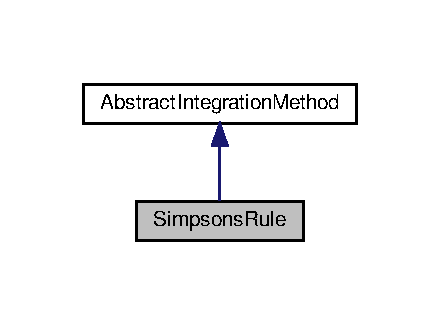
\includegraphics[width=211pt]{class_simpsons_rule__inherit__graph}
\end{center}
\end{figure}


Collaboration diagram for Simpsons\+Rule\+:\nopagebreak
\begin{figure}[H]
\begin{center}
\leavevmode
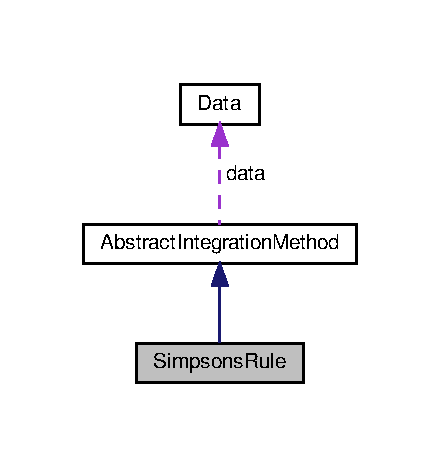
\includegraphics[width=211pt]{class_simpsons_rule__coll__graph}
\end{center}
\end{figure}
\subsection*{Public Member Functions}
\begin{DoxyCompactItemize}
\item 
\mbox{\Hypertarget{class_simpsons_rule_af880433d19d6041cdedb081b542a195b}\label{class_simpsons_rule_af880433d19d6041cdedb081b542a195b}} 
\hyperlink{class_simpsons_rule_af880433d19d6041cdedb081b542a195b}{Simpsons\+Rule} (\hyperlink{struct_data}{Data} data, Eigen\+::\+Vector\+Xcd($\ast$f)(double x, double y, Eigen\+::\+Matrix\+Xcd coeff))
\begin{DoxyCompactList}\small\item\em Initialiser setting the data as a \hyperlink{struct_data}{Data} struct and also the function to integrate. \end{DoxyCompactList}\item 
Eigen\+::\+Vector\+Xcd \hyperlink{class_simpsons_rule_a9925b07e44be9fc1644d3cbeb742078c}{Solve} ()
\begin{DoxyCompactList}\small\item\em Method to compute approximate value of the 2D or 1D integral with Simpson\textquotesingle{}s Rule. \end{DoxyCompactList}\end{DoxyCompactItemize}
\subsection*{Additional Inherited Members}


\subsection{Detailed Description}
Class implementing the Simpson\textquotesingle{}s Rule approximation of integrals in 2D or 1D. 

Takes as input a \hyperlink{struct_data}{Data} struct and implements a \hyperlink{class_simpsons_rule_a9925b07e44be9fc1644d3cbeb742078c}{Solve()} method returning the 2D or 1D Simpson\textquotesingle{}s Rule approximation of the integral 

\subsection{Member Function Documentation}
\mbox{\Hypertarget{class_simpsons_rule_a9925b07e44be9fc1644d3cbeb742078c}\label{class_simpsons_rule_a9925b07e44be9fc1644d3cbeb742078c}} 
\index{Simpsons\+Rule@{Simpsons\+Rule}!Solve@{Solve}}
\index{Solve@{Solve}!Simpsons\+Rule@{Simpsons\+Rule}}
\subsubsection{\texorpdfstring{Solve()}{Solve()}}
{\footnotesize\ttfamily Eigen\+::\+Vector\+Xcd Simpsons\+Rule\+::\+Solve (\begin{DoxyParamCaption}{ }\end{DoxyParamCaption})\hspace{0.3cm}{\ttfamily [virtual]}}



Method to compute approximate value of the 2D or 1D integral with Simpson\textquotesingle{}s Rule. 

Takes as input a \hyperlink{struct_data}{Data} struct and implements a \hyperlink{class_simpsons_rule_a9925b07e44be9fc1644d3cbeb742078c}{Solve()} method returning the 2D or 1D Simpson\textquotesingle{}s Rule approximation of the integral \begin{eqnarray*} I \approx & \frac{h_x h_y}{36} \left[ f(x_0, y_0)+f(x_0,y_f)+f(x_f,y_0)+f(x_f,y_f) \right.\\ & + 4 \left( \sum_{i=1}^{n_y} \left[f(x_0, y_{2i-1})+f(x_f,y_{2i-1})\right] + \sum_{j=1}^{n_x} \left[f(x_{2j-1}, y_0)+f(x_{2j-1},y_f)\right] \right)\\ & + 2 \left( \sum_{i=1}^{n_y-1} \left[f(x_0, y_{2i})+f(x_f,y_{2i})\right] + \sum_{j=1}^{n_x-1} \left[f(x_{2j}, y_0)+f(x_{2j},y_f)\right] \right) \\ & + 4 \left( \sum_{i=1}^{n_y-1} \sum_{j=1}^{n_x-1} f(x_{2j}, y_{2i}) \right) + 16 \left( \sum_{i=1}^{n_y} \sum_{j=1}^{n_x} f(x_{2j-1}, y_{2i-1}) \right) \\ & \left. +8 \left( \sum_{i=1}^{n_y} \sum_{j=1}^{n_x-1} f(x_{2j}, y_{2i-1}) + \sum_{i=1}^{n_y-1} \sum_{j=1}^{n_x} f(x_{2j-1}, y_{2i}) \right) \right] \end{eqnarray*}

\begin{DoxyReturn}{Returns}
The complex vector result of the integral approximation 
\end{DoxyReturn}


Implements \hyperlink{class_abstract_integration_method_af76e5bdce7d0b139d07e920fa29c1c34}{Abstract\+Integration\+Method}.



The documentation for this class was generated from the following files\+:\begin{DoxyCompactItemize}
\item 
Simpsons\+Rule.\+h\item 
Simpsons\+Rule.\+cpp\end{DoxyCompactItemize}

\hypertarget{class_trapezoidal_rule}{}\section{Trapezoidal\+Rule Class Reference}
\label{class_trapezoidal_rule}\index{Trapezoidal\+Rule@{Trapezoidal\+Rule}}


Class implementing the Trapezoidal Rule approximation of integrals in 2D or 1D.  




{\ttfamily \#include $<$Trapezoidal\+Rule.\+h$>$}



Inheritance diagram for Trapezoidal\+Rule\+:\nopagebreak
\begin{figure}[H]
\begin{center}
\leavevmode
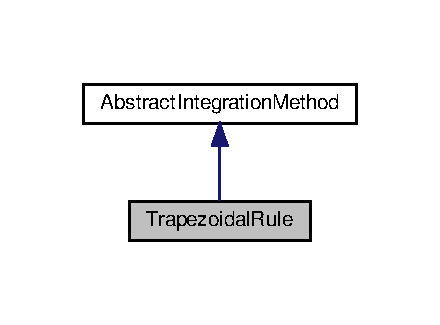
\includegraphics[width=211pt]{class_trapezoidal_rule__inherit__graph}
\end{center}
\end{figure}


Collaboration diagram for Trapezoidal\+Rule\+:\nopagebreak
\begin{figure}[H]
\begin{center}
\leavevmode
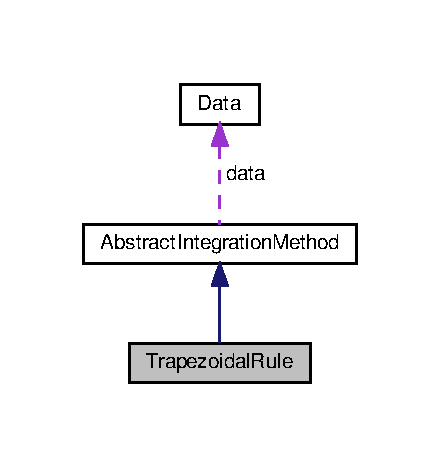
\includegraphics[width=211pt]{class_trapezoidal_rule__coll__graph}
\end{center}
\end{figure}
\subsection*{Public Member Functions}
\begin{DoxyCompactItemize}
\item 
\mbox{\Hypertarget{class_trapezoidal_rule_a950f29db214b348a6dd9c03bf05fadac}\label{class_trapezoidal_rule_a950f29db214b348a6dd9c03bf05fadac}} 
\hyperlink{class_trapezoidal_rule_a950f29db214b348a6dd9c03bf05fadac}{Trapezoidal\+Rule} (\hyperlink{struct_data}{Data} \&data, Eigen\+::\+Vector\+Xcd($\ast$f)(double x, double y, Eigen\+::\+Matrix\+Xcd \&coeff))
\begin{DoxyCompactList}\small\item\em Initialiser setting the data as a \hyperlink{struct_data}{Data} struct and also the function to integrate. \end{DoxyCompactList}\item 
Eigen\+::\+Vector\+Xcd \hyperlink{class_trapezoidal_rule_ae822d86948bdc8876bf524cd620e11b8}{Solve} ()
\begin{DoxyCompactList}\small\item\em Method to compute approximate value of the 2D or 1D integral with Trapezoidal Rule. \end{DoxyCompactList}\end{DoxyCompactItemize}
\subsection*{Additional Inherited Members}


\subsection{Detailed Description}
Class implementing the Trapezoidal Rule approximation of integrals in 2D or 1D. 

Takes as input a \hyperlink{struct_data}{Data} struct and implements a \hyperlink{class_trapezoidal_rule_ae822d86948bdc8876bf524cd620e11b8}{Solve()} method returning the 2D or 1D Trapezoidal Rule approximation of the integral 

\subsection{Member Function Documentation}
\mbox{\Hypertarget{class_trapezoidal_rule_ae822d86948bdc8876bf524cd620e11b8}\label{class_trapezoidal_rule_ae822d86948bdc8876bf524cd620e11b8}} 
\index{Trapezoidal\+Rule@{Trapezoidal\+Rule}!Solve@{Solve}}
\index{Solve@{Solve}!Trapezoidal\+Rule@{Trapezoidal\+Rule}}
\subsubsection{\texorpdfstring{Solve()}{Solve()}}
{\footnotesize\ttfamily Eigen\+::\+Vector\+Xcd Trapezoidal\+Rule\+::\+Solve (\begin{DoxyParamCaption}{ }\end{DoxyParamCaption})\hspace{0.3cm}{\ttfamily [virtual]}}



Method to compute approximate value of the 2D or 1D integral with Trapezoidal Rule. 

Takes as input a \hyperlink{struct_data}{Data} struct and implements a \hyperlink{class_trapezoidal_rule_ae822d86948bdc8876bf524cd620e11b8}{Solve()} method returning the 2D or 1D Trapezoidal Rule approximation of the integral \begin{eqnarray*} I \approx& \frac{h_x h_y}{4} \left[ f(x_0, y_0)+f(x_0,y_f)+f(x_f,y_0)+f(x_f,y_f) + 4 \sum_{i=1}^{n_y-1} \sum_{j=1}^{n_x-1} f(x_j, y_i) \right.\\ & \left. + 2 \sum_{i=1}^{n_y-1} \left(f(x_0, y_i)+f(x_f,y_i)\right) + 2 \sum_{j=1}^{n_x-1} \left(f(x_j, y_0)+f(x_j,y_f)\right) \right] \end{eqnarray*}

\begin{DoxyReturn}{Returns}
The complex vector result of the integral approximation 
\end{DoxyReturn}


Implements \hyperlink{class_abstract_integration_method_af76e5bdce7d0b139d07e920fa29c1c34}{Abstract\+Integration\+Method}.



The documentation for this class was generated from the following files\+:\begin{DoxyCompactItemize}
\item 
Trapezoidal\+Rule.\+h\item 
Trapezoidal\+Rule.\+cpp\end{DoxyCompactItemize}

\hypertarget{class_txt_reader}{}\section{Txt\+Reader Class Reference}
\label{class_txt_reader}\index{Txt\+Reader@{Txt\+Reader}}


Inheritance diagram for Txt\+Reader\+:\nopagebreak
\begin{figure}[H]
\begin{center}
\leavevmode
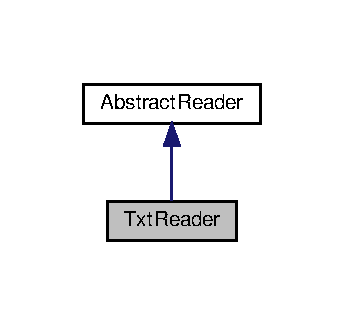
\includegraphics[width=165pt]{class_txt_reader__inherit__graph}
\end{center}
\end{figure}


Collaboration diagram for Txt\+Reader\+:\nopagebreak
\begin{figure}[H]
\begin{center}
\leavevmode
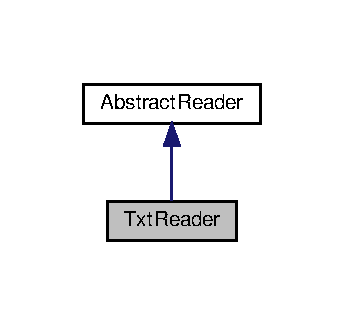
\includegraphics[width=165pt]{class_txt_reader__coll__graph}
\end{center}
\end{figure}
\subsection*{Public Member Functions}
\begin{DoxyCompactItemize}
\item 
\mbox{\Hypertarget{class_txt_reader_acbef0ef9c6034581d76a3b9e305f1508}\label{class_txt_reader_acbef0ef9c6034581d76a3b9e305f1508}} 
{\bfseries Txt\+Reader} (std\+::string filename)
\item 
\hyperlink{struct_data}{Data} \hyperlink{class_txt_reader_a30786dcd83c2f24dd26e83cb5fd934ab}{Output\+Data} ()
\begin{DoxyCompactList}\small\item\em Method to compute data as \hyperlink{struct_data}{Data} struct from file. \end{DoxyCompactList}\end{DoxyCompactItemize}
\subsection*{Additional Inherited Members}


\subsection{Member Function Documentation}
\mbox{\Hypertarget{class_txt_reader_a30786dcd83c2f24dd26e83cb5fd934ab}\label{class_txt_reader_a30786dcd83c2f24dd26e83cb5fd934ab}} 
\index{Txt\+Reader@{Txt\+Reader}!Output\+Data@{Output\+Data}}
\index{Output\+Data@{Output\+Data}!Txt\+Reader@{Txt\+Reader}}
\subsubsection{\texorpdfstring{Output\+Data()}{OutputData()}}
{\footnotesize\ttfamily \hyperlink{struct_data}{Data} Txt\+Reader\+::\+Output\+Data (\begin{DoxyParamCaption}{ }\end{DoxyParamCaption})\hspace{0.3cm}{\ttfamily [virtual]}}



Method to compute data as \hyperlink{struct_data}{Data} struct from file. 

\begin{DoxyReturn}{Returns}
A \hyperlink{struct_data}{Data} object read from the the file 
\end{DoxyReturn}


Implements \hyperlink{class_abstract_reader_a14b05f156920be0cfa0cabdb1c6c1267}{Abstract\+Reader}.



The documentation for this class was generated from the following files\+:\begin{DoxyCompactItemize}
\item 
Txt\+Reader.\+h\item 
Txt\+Reader.\+cpp\end{DoxyCompactItemize}

%--- End generated contents ---

% Index
\backmatter
\newpage
\phantomsection
\clearemptydoublepage
\addcontentsline{toc}{chapter}{Index}
\printindex

\end{document}
